\documentclass[12pt]{article}

\setlength{\parskip}{1em}

\usepackage[T1]{fontenc}
\usepackage[a4paper, margin=0.7in]{geometry}
\usepackage{amsfonts}
\usepackage{mathabx}
\usepackage{listings}
\usepackage{xcolor}
\usepackage{subcaption}
\usepackage{multirow}
\usepackage{makecell}
\usepackage{graphicx}
\usepackage{float}
\usepackage{pdfpages}
\usepackage[french]{babel}

\usepackage{hyperref}
\hypersetup{
  colorlinks=true,
  linkcolor=blue,
  urlcolor=blue,
  pdftitle={AP4B Project: Power Sim}
}

\definecolor{bgColor}{rgb}{0.95,0.95,0.92}
\lstdefinestyle{Java}{
    backgroundcolor=\color{bgColor},
    commentstyle=\color{gray},
    keywordstyle=\color{magenta},
    numberstyle=\tiny\color{gray},
    stringstyle=\color{purple},
    basicstyle=\footnotesize,
    breakatwhitespace=false,
    breaklines=true,
    captionpos=b,
    keepspaces=true,
    numbers=left,
    numbersep=5pt,
    showspaces=false,
    showstringspaces=false,
    showtabs=false,
    tabsize=2,
    language=JAVA
}

\graphicspath{{report/}}

\title{Projet d'AP4B: Power Sim}
\author{
    Osée Tchappi \\
    Adrien Burgun \\
    Tarabai Gambara \\
    Jiang YiWen
}
\date{Automne 2021}

\begin{document}
\maketitle

\begin{abstract}
    Pour ce projet d'AP4B, nous avons décidé de choisir le sujet "Power Sim".

    Ce document décrit notre démarche de conception du projet, à la vue de l'implémentation du jeu en Java dans les semaines à venir.

    Lors de cette démarche de conception, nous avons été amenés à écrire des diagrammes UML, ceux-cis sont également présentés dans ce document.

    Certains diagrammes (Cas d'utilisation - Section~\ref{sec:usecase} et Diagramme de Classe - Section~\ref{sec:class}) ont été découpés en plusieurs sous-diagrammes pour la lisibilité; les diagrammes complets, ainsi que le code source de ce rapport, peuvent être trouvés sur GitHub: \url{https://github.com/adri326/ap4b-project/}.
\end{abstract}

\newpage
\tableofcontents
\newpage

\section{Introduction}

Nous avons choisi parmis les sujets proposés celui intitulé \og Power Sim \fg, car il nous a plus inspiré et qu'il nous donne plus de liberté en termes de systèmes que nous souhaitons mettre en place.

Nous nous sommes rassemblé chaque vendredi pour mettre en commun notre travail et pour distribuer le travail pour la semaine à venir.
Nous avons d'abords collecté des idées indépendamment, puis nous avons construit un diagramme de cas d'utilisation et mis en place la repository pour le projet.

Nous avons ensuite travaillé en parallèle sur différents diagrammes: le diagramme de classe, les diagrammes de séquence, la description textuelle des cas d'utilisation et le diagramme de communication.

Nous avons décidé de modéliser le sujet de la manière suivante:

\begin{itemize}
    \item Le joueur construit une ville, qui est constituée de bâtiments se trouvant sur une grille.
    \item Le joueur peut placer, modifier et supprimer des bâtiments.
    \item Des habitants s'installent lorsque des resources (éléctricité, routes) sont disponibles: ils construisent des maisons et d'autres bâtiments là où il y a de la place.
    \item L'accent est placé sur les simulations faisant vivre la ville: la pollution, le transfert de resources entre les bâtiments et la satisfaction des habitants sont simulés.
    \item Alors que la ville grandit et que le joueur construit des bâtiments, des technologies sont débloquées, le permettant d'améliorer des bâtiments ou de placer de nouveaux bâtiments: de cette manière, le joueur peut produire de l'énergie plus proprement et plus efficacement.
\end{itemize}

\section{Cas d'utilisations}
\label{sec:usecase}

Notre phase de conception a débutté avec la mise en place d'un diagramme de cas d'utilisation.

Trois acteurs se dessinent:

\begin{itemize}
    \item \textbf{Le joueur}; ses interactions sont marquées par des entrées clavier/souris, ainsi que son besoin de percevoir les informations du jeu. Le joueur place les bâtiments qu'il veut, il choisit les options, il observe la ville évoluer.
    \item \textbf{La simulation}; celle-ci a des interactions à caractère périodique avec le jeu: sa plus importante est l'étape de simulation, qui est divisée en différents aspects du jeu. (pollution, immigration, production d'énergie, etc.)
    \item \textbf{La banque}; celle-ci gère l'argent du joueur: elle offre au joueur un solde initial, ainsi que des prêts s'il n'a plus d'argent.
\end{itemize}

\newpage

\begin{figure}[H]
    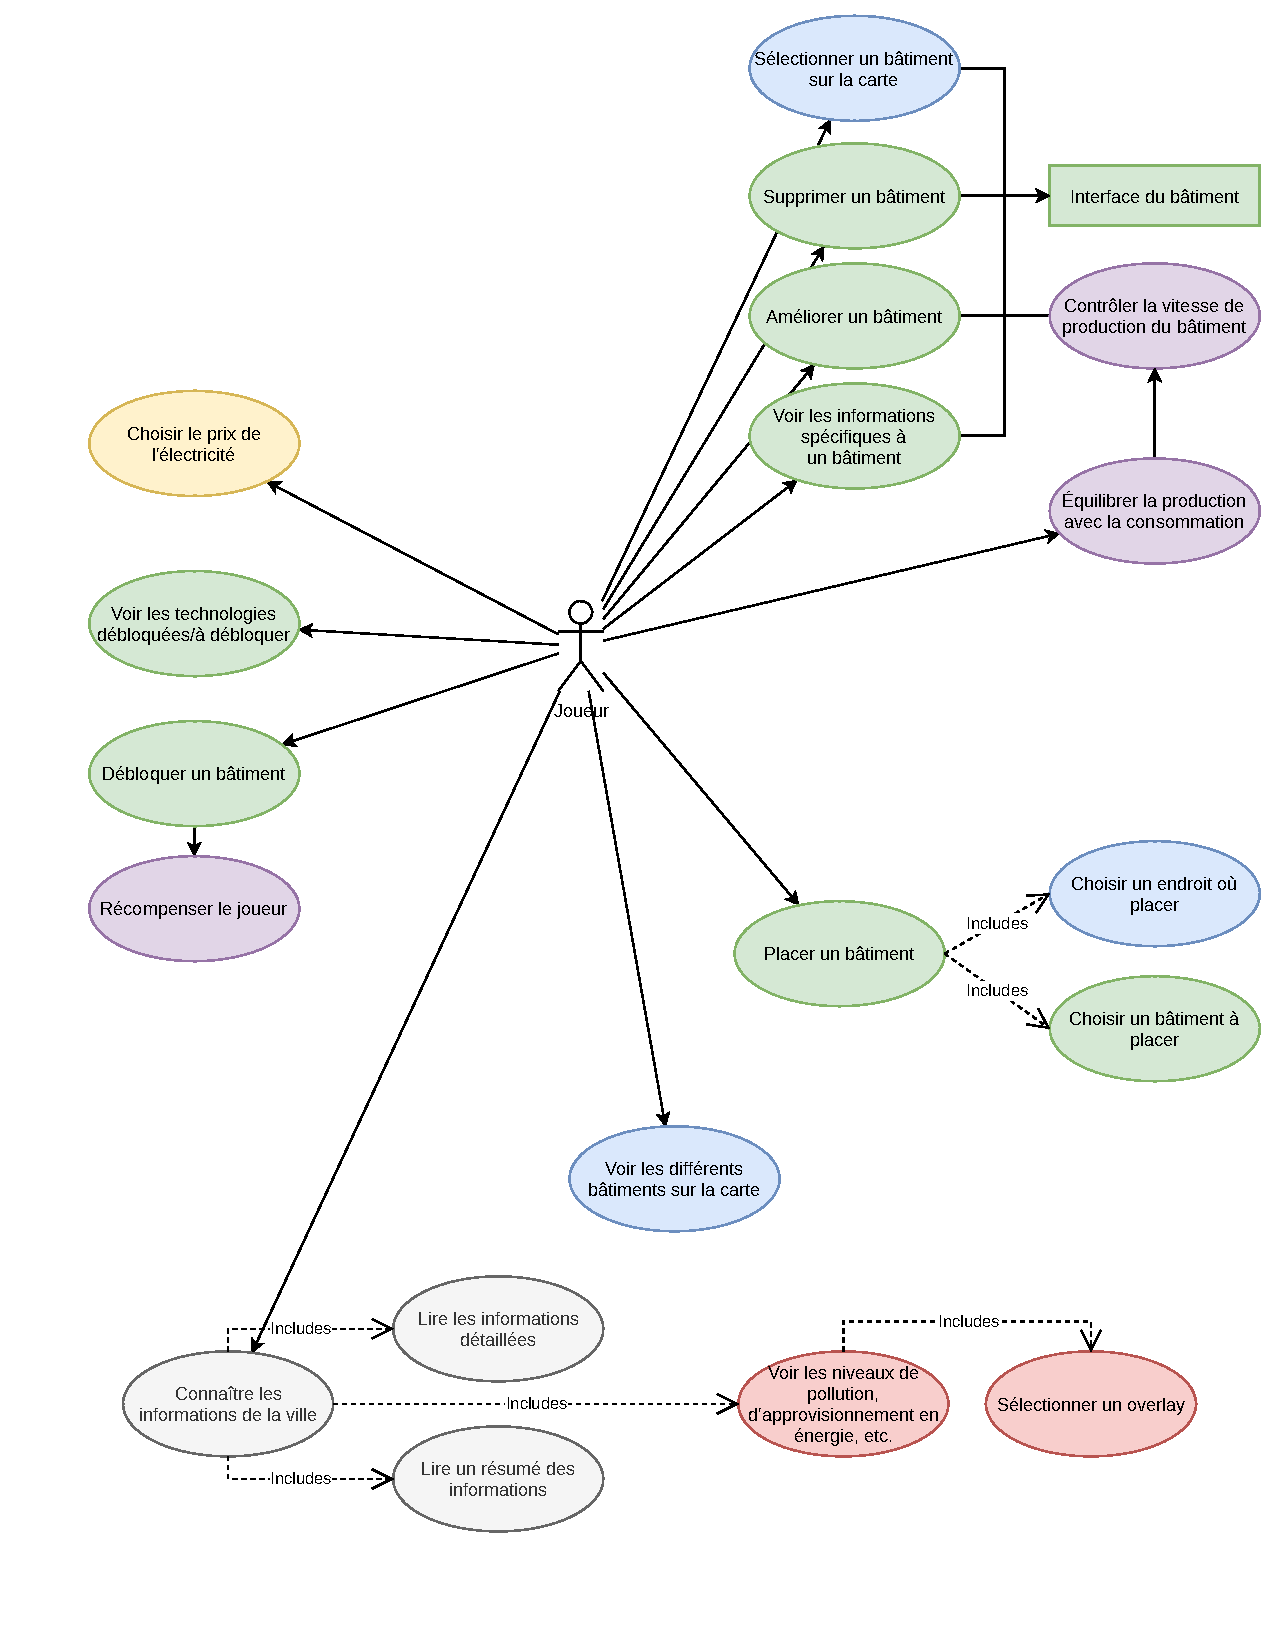
\includegraphics[width=\textwidth]{uml-usecases-Page-2}
    \caption{Les cas d'utilisation associés au joueur \label{fig:usecase-player}}
\end{figure}

\begin{figure}[H]
    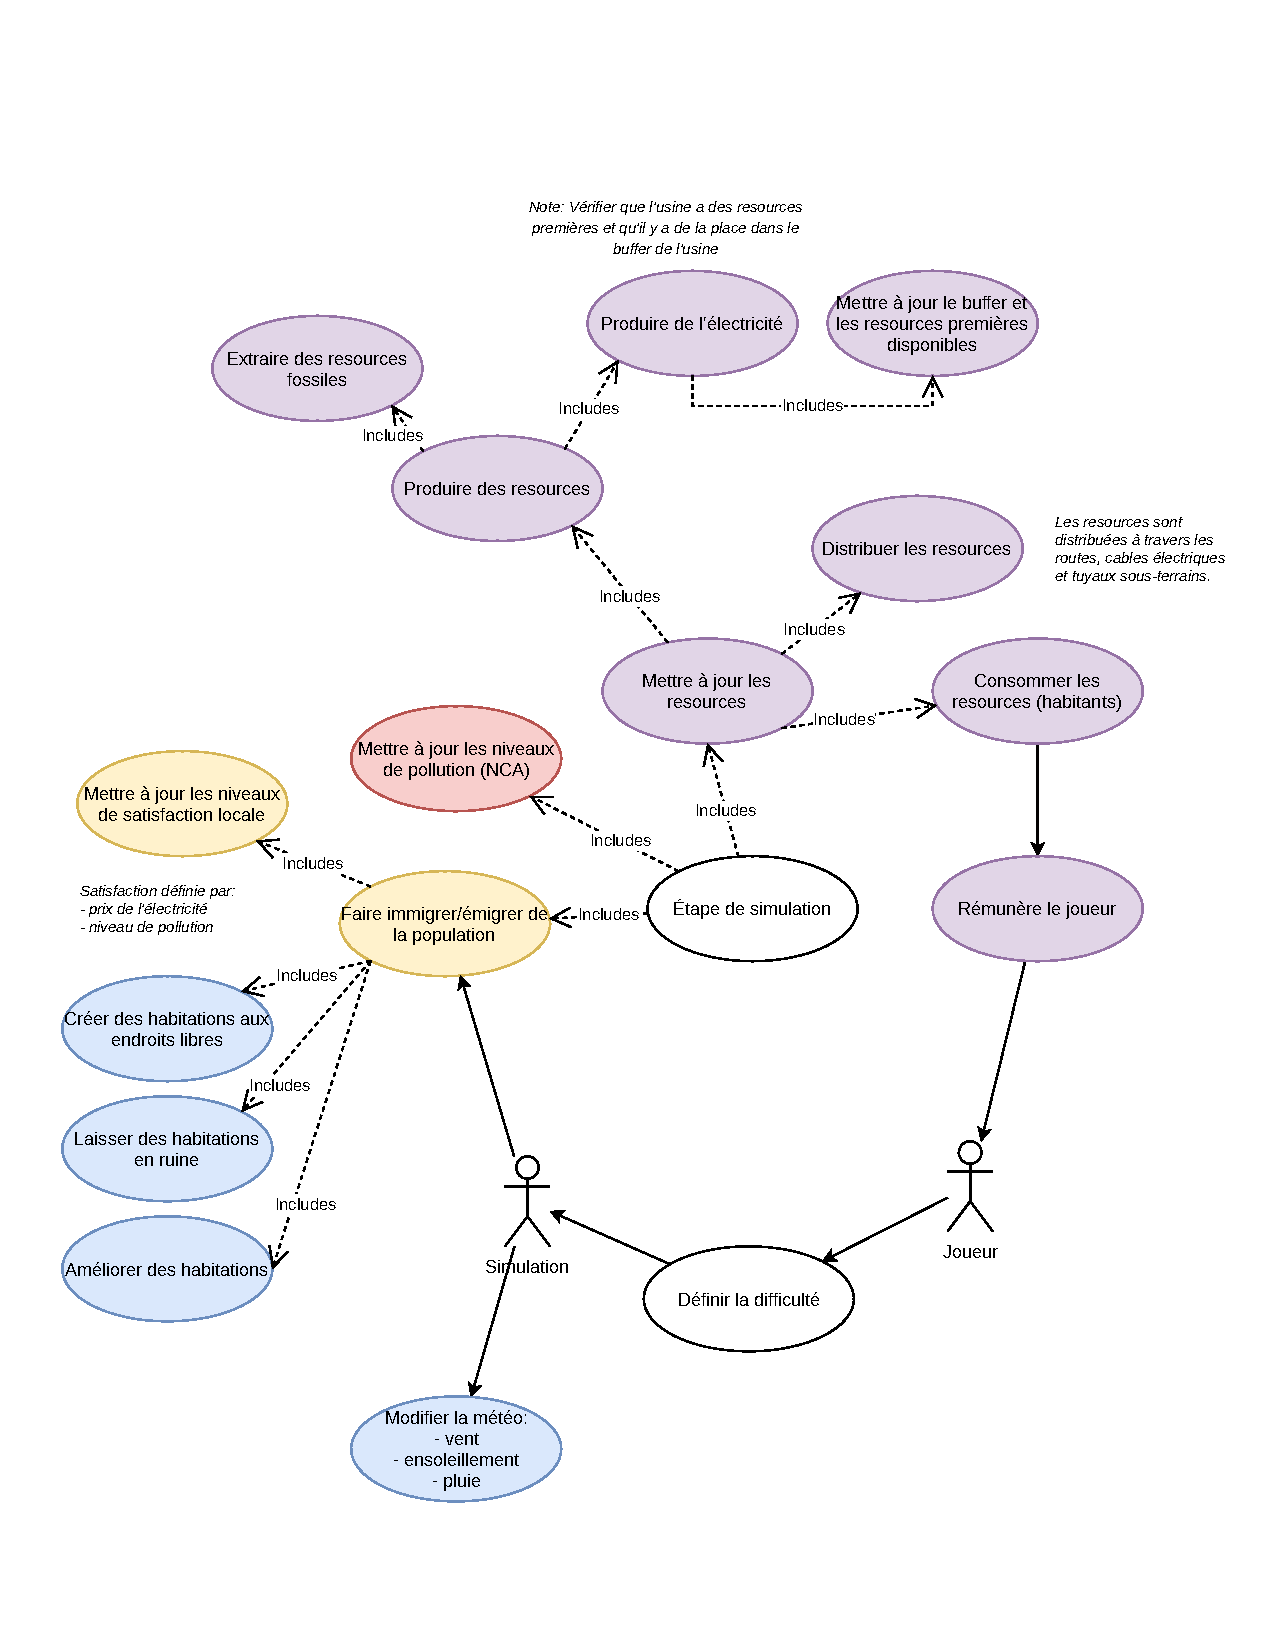
\includegraphics[width=\textwidth]{uml-usecases-Page-3}
    \caption{Les cas d'utilisation associés à la simulation \label{fig:usecase-simulation}}
\end{figure}

\begin{figure}[H]
    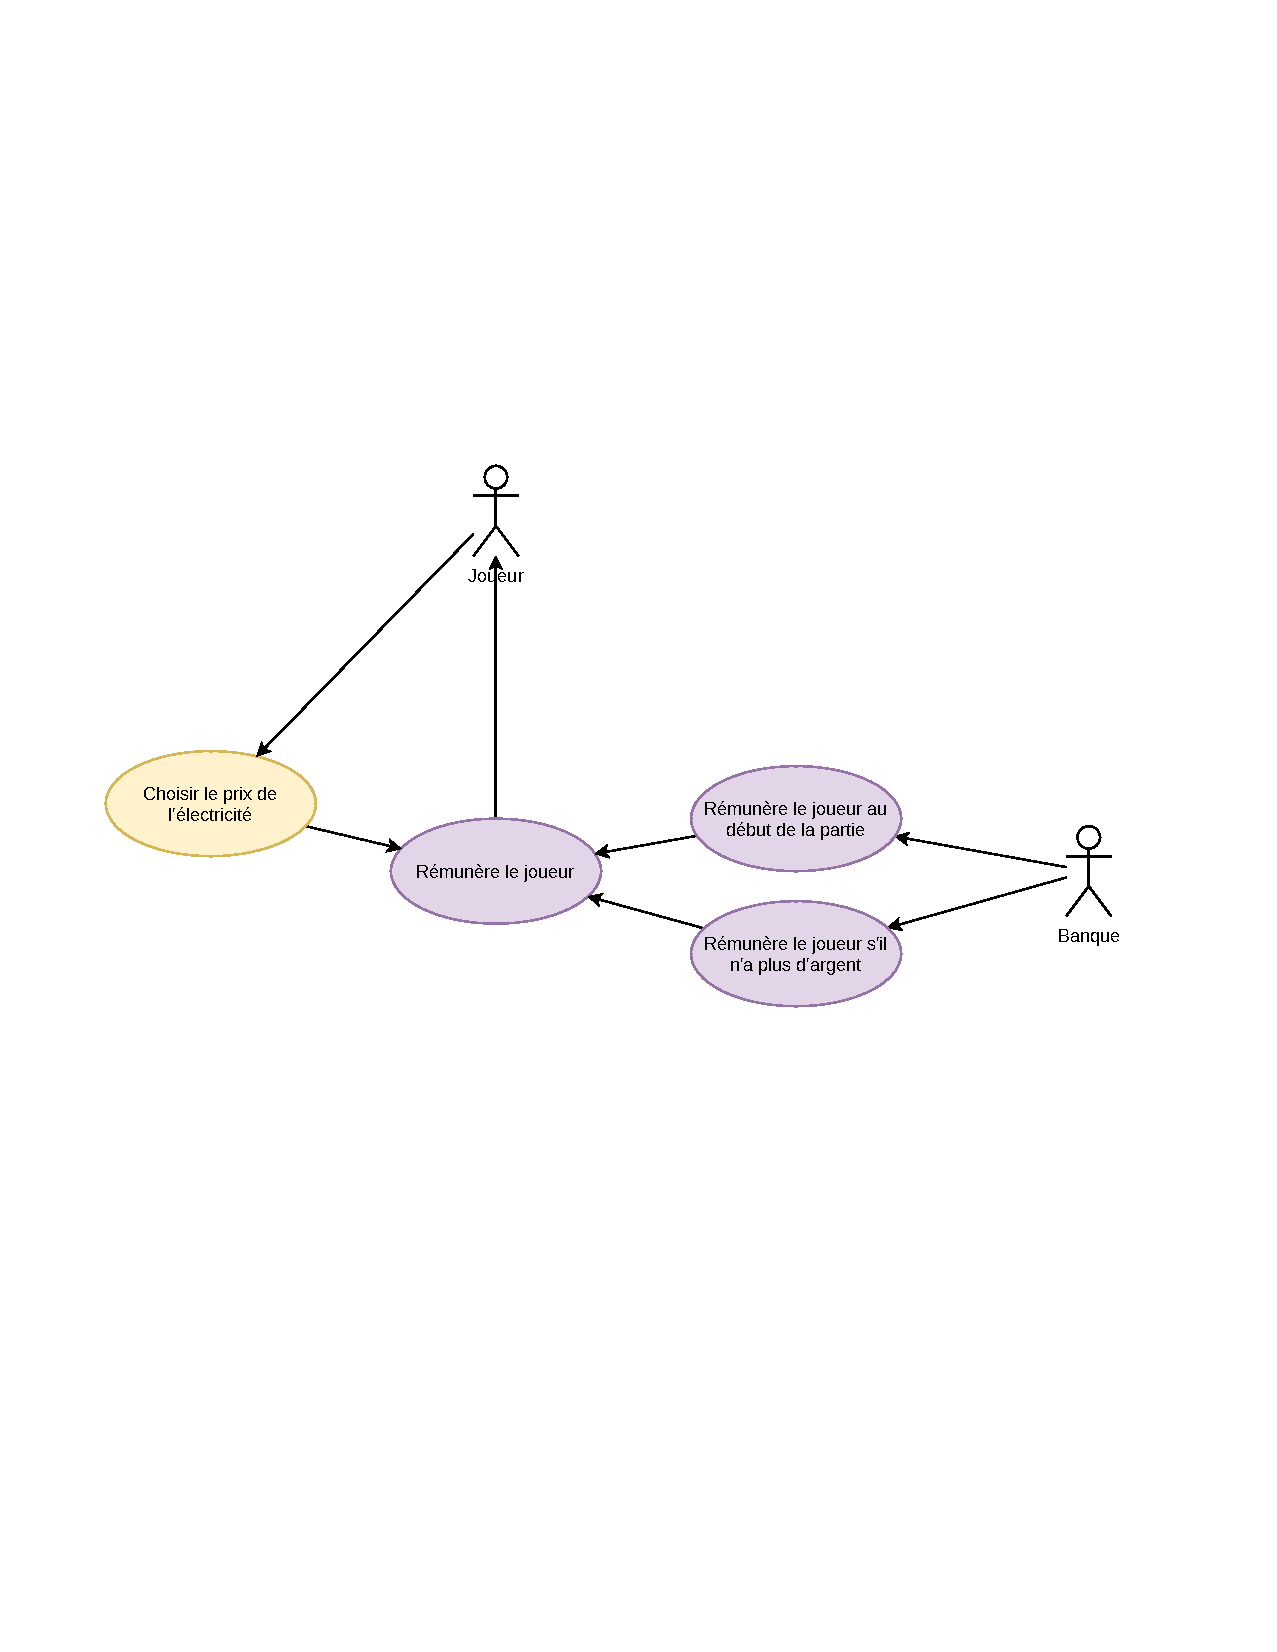
\includegraphics[width=\textwidth]{uml-usecases-Page-4}
    \caption{Les cas d'utilisation associés à la banque \label{fig:usecase-bank}}
\end{figure}


\section{Diagramme de Classe}
\label{sec:class}

Nous avons construit un diagramme de classe, implémentant les besoins émis dans le diagramme de cas d'utilisation et servant de base aux diagrammes de séquences venant par la suite.

Dans cette conception du projet, la classe \texttt{GameState} est la classe principale de la méchanique du jeu: celle-ci stoque l'entièreté des informations d'une partie.
Les différents composants de cette classe correspondent aux différents besoins du projet:

\begin{itemize}
    \item La classe \texttt{Tile} (Figure~\ref{fig:tile}, contenue dans la classe \texttt{Map}) est commune à tous les bâtiments posés sur l'espace de jeu: celle-ci est étendue pour implémenter la logique et les spécificités des différents bâtiments (Figure~\ref{fig:factory}).
    \item La classe \texttt{Bank} gère la partie "banque": rémunérer le joueur au début, faire un prêt, etc.
    \item La classe \texttt{Simulation} gère le coeur de la simulation du jeu: l'immigration, la génération de resources et la pollution.
    \item La classe \texttt{Weather} contient une petite simulation de météo et du cycle jour/nuit.
    \item La classe \texttt{TechTree} (Figure~\ref{fig:techtree}) contient les technologies que le joueur débloque au fil de la partie: celles-cis sont caractérisées par des pré-requis (\texttt{Requirement}) et des récompenses (\texttt{Reward}).
\end{itemize}

Les classes spécifiques à la partie graphisme sont incluses dans ce rapport mais seront amenées à être modifiées et étendues lors de la phase d'implémentation du projet. Celles-cis se trouve dans la Figure~\ref{fig:application}

\begin{figure}[H]
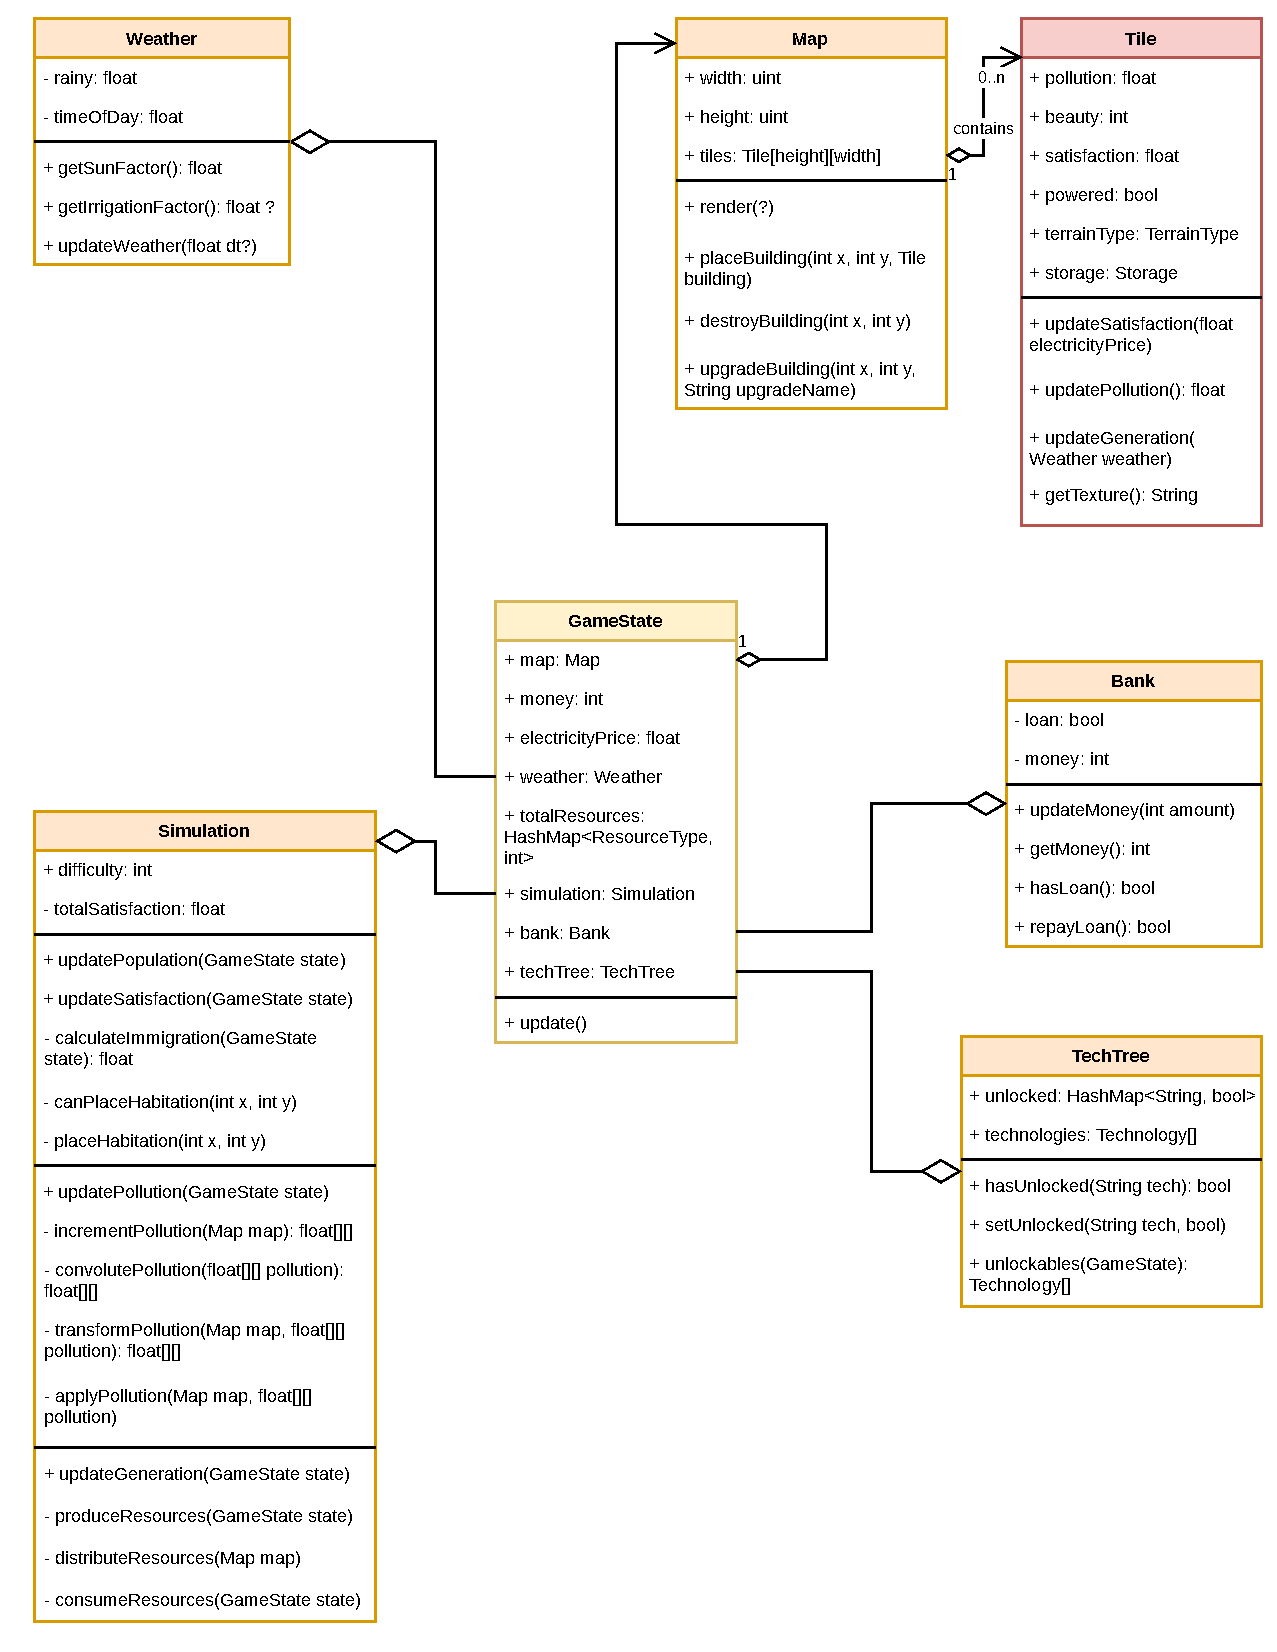
\includegraphics[width=\textwidth]{uml-classes-Page-2}
\caption{La classe principale \texttt{GameState} et les classes qu'elle contient.\label{fig:gamestate}}
\end{figure}

\begin{figure}[H]
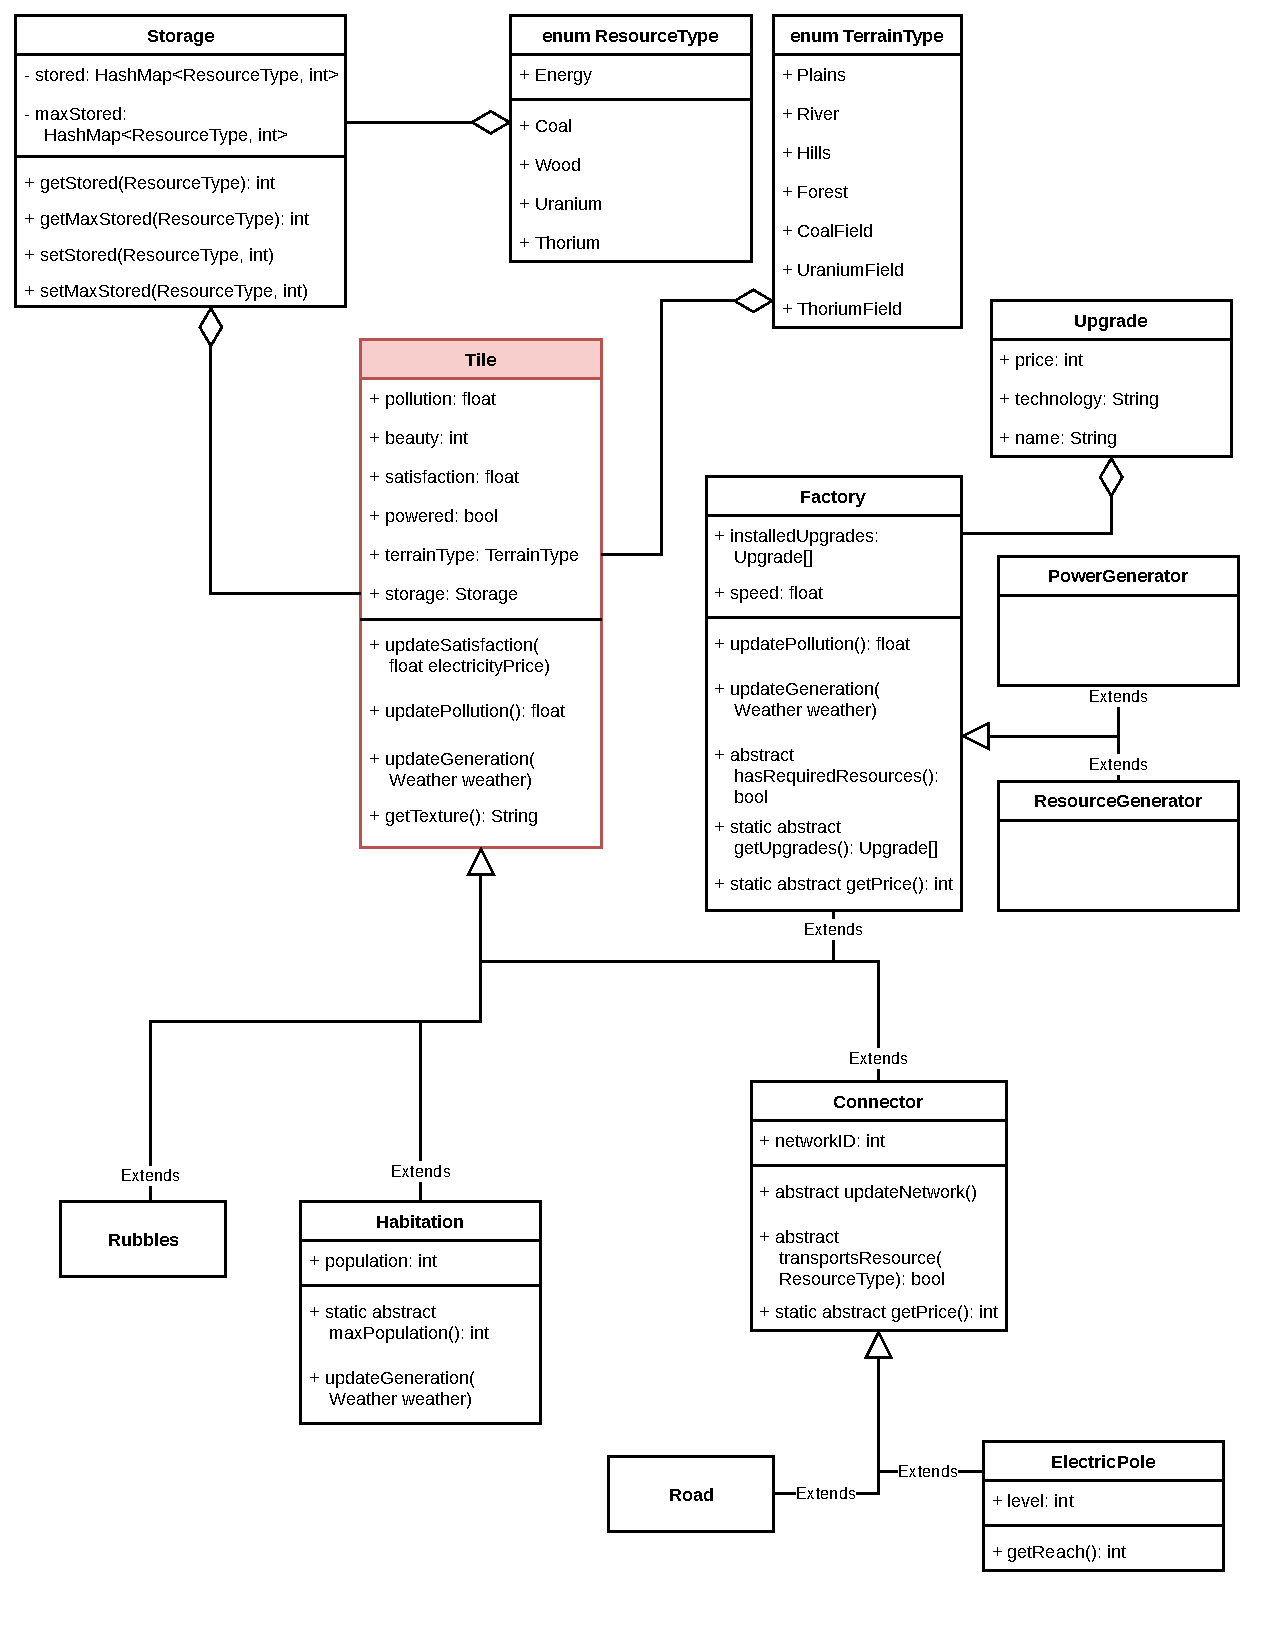
\includegraphics[width=\textwidth]{uml-classes-Page-3}
\caption{La classe \texttt{Tile} et ses principaux descendants.\label{fig:tile}}
\end{figure}

\begin{figure}[H]
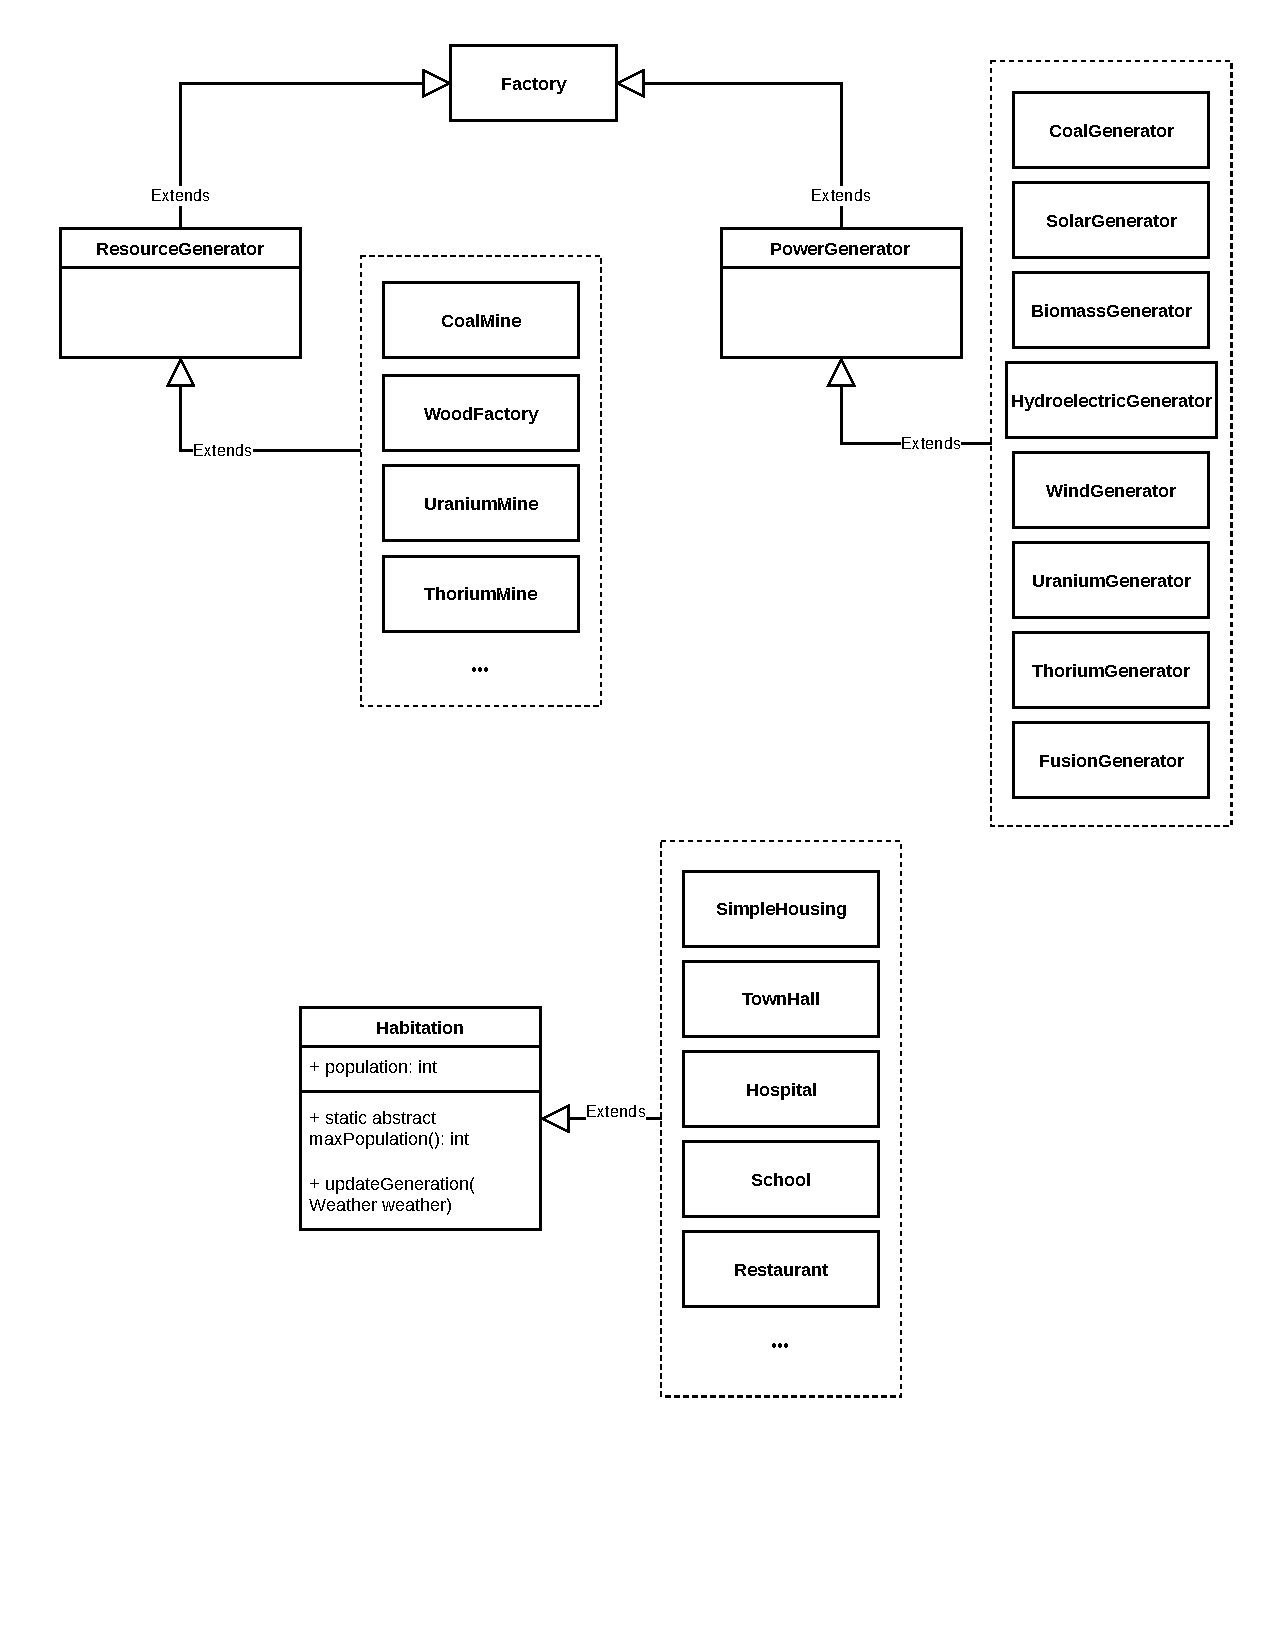
\includegraphics[width=\textwidth]{uml-classes-Page-4}
\caption{Détail de Figure~\ref{fig:tile}: les classes descendant de \texttt{Factory} et de \texttt{Habitation}.\label{fig:factory}}
\end{figure}

\begin{figure}[H]
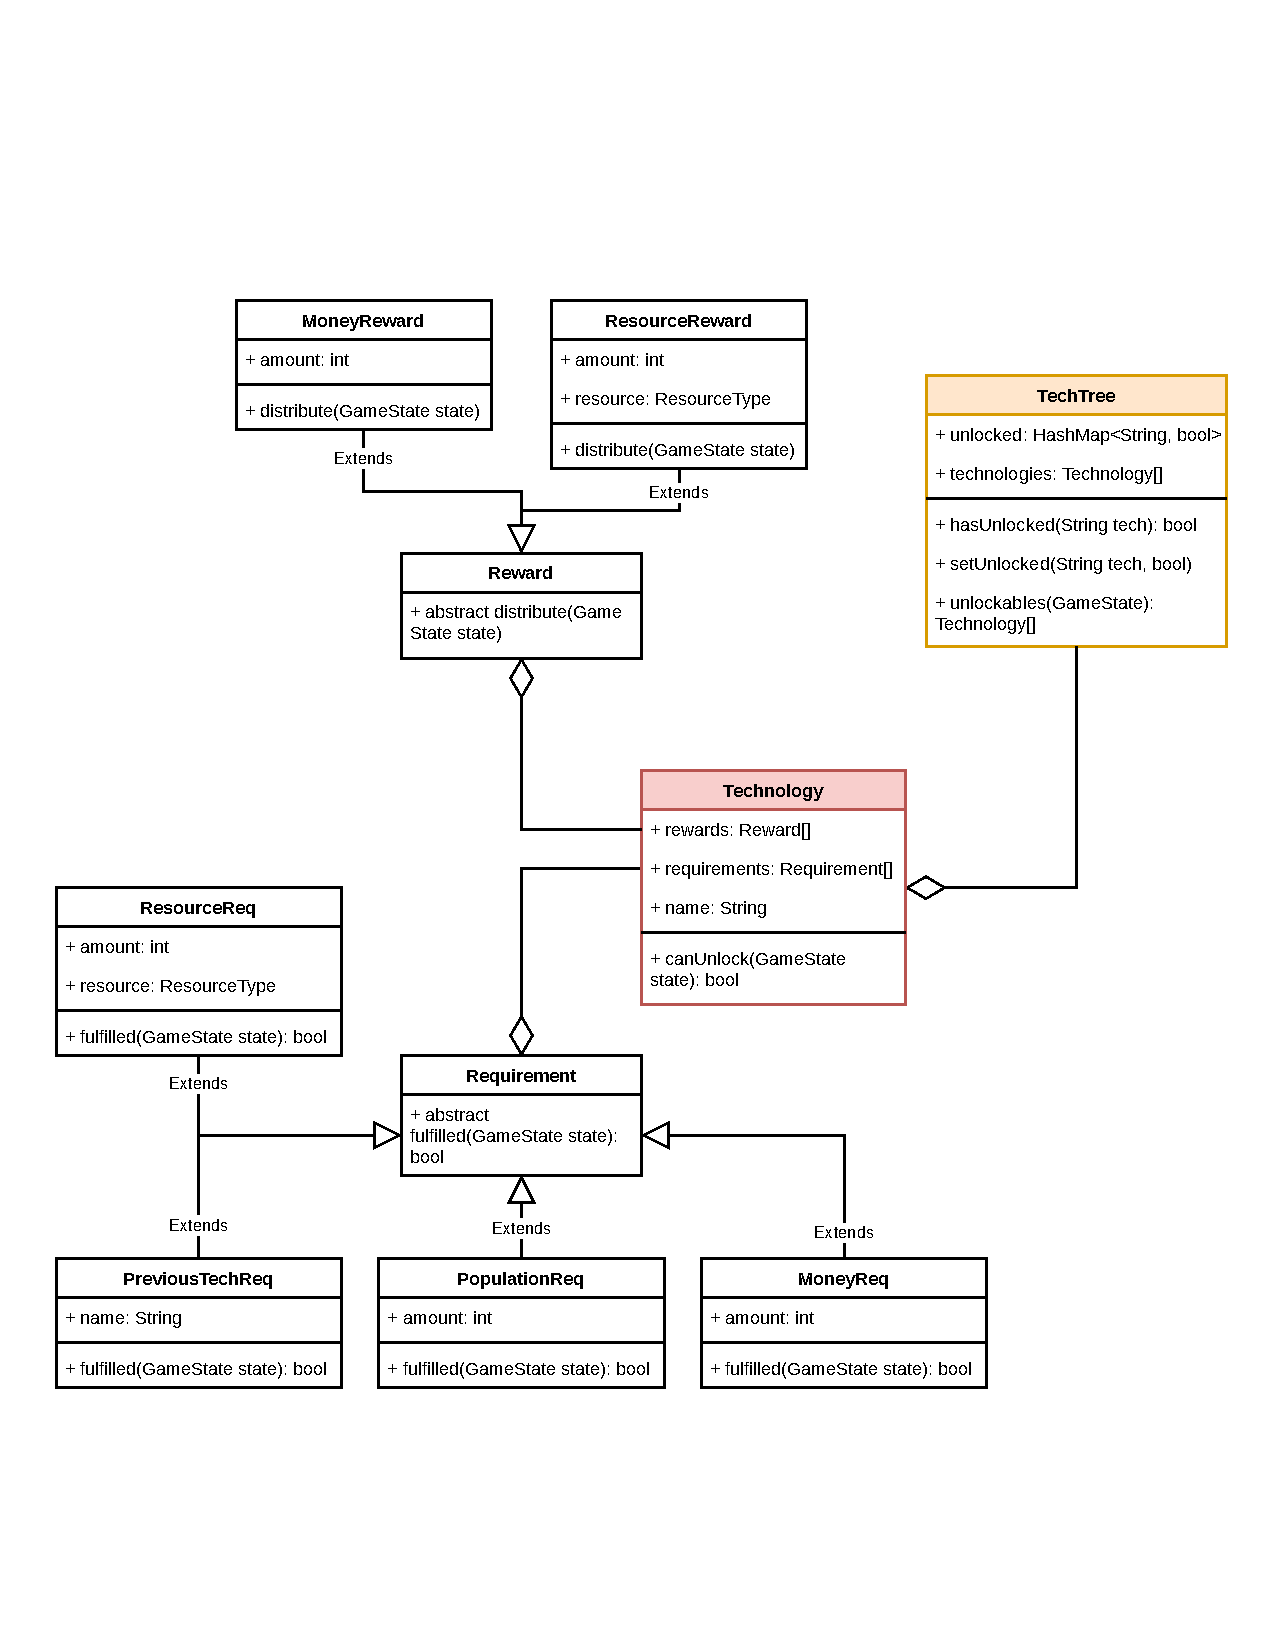
\includegraphics[width=\textwidth]{uml-classes-Page-5}
\caption{La classe \texttt{TechTree} et ses principaux descendants.\label{fig:techtree}}
\end{figure}

\begin{figure}[H]
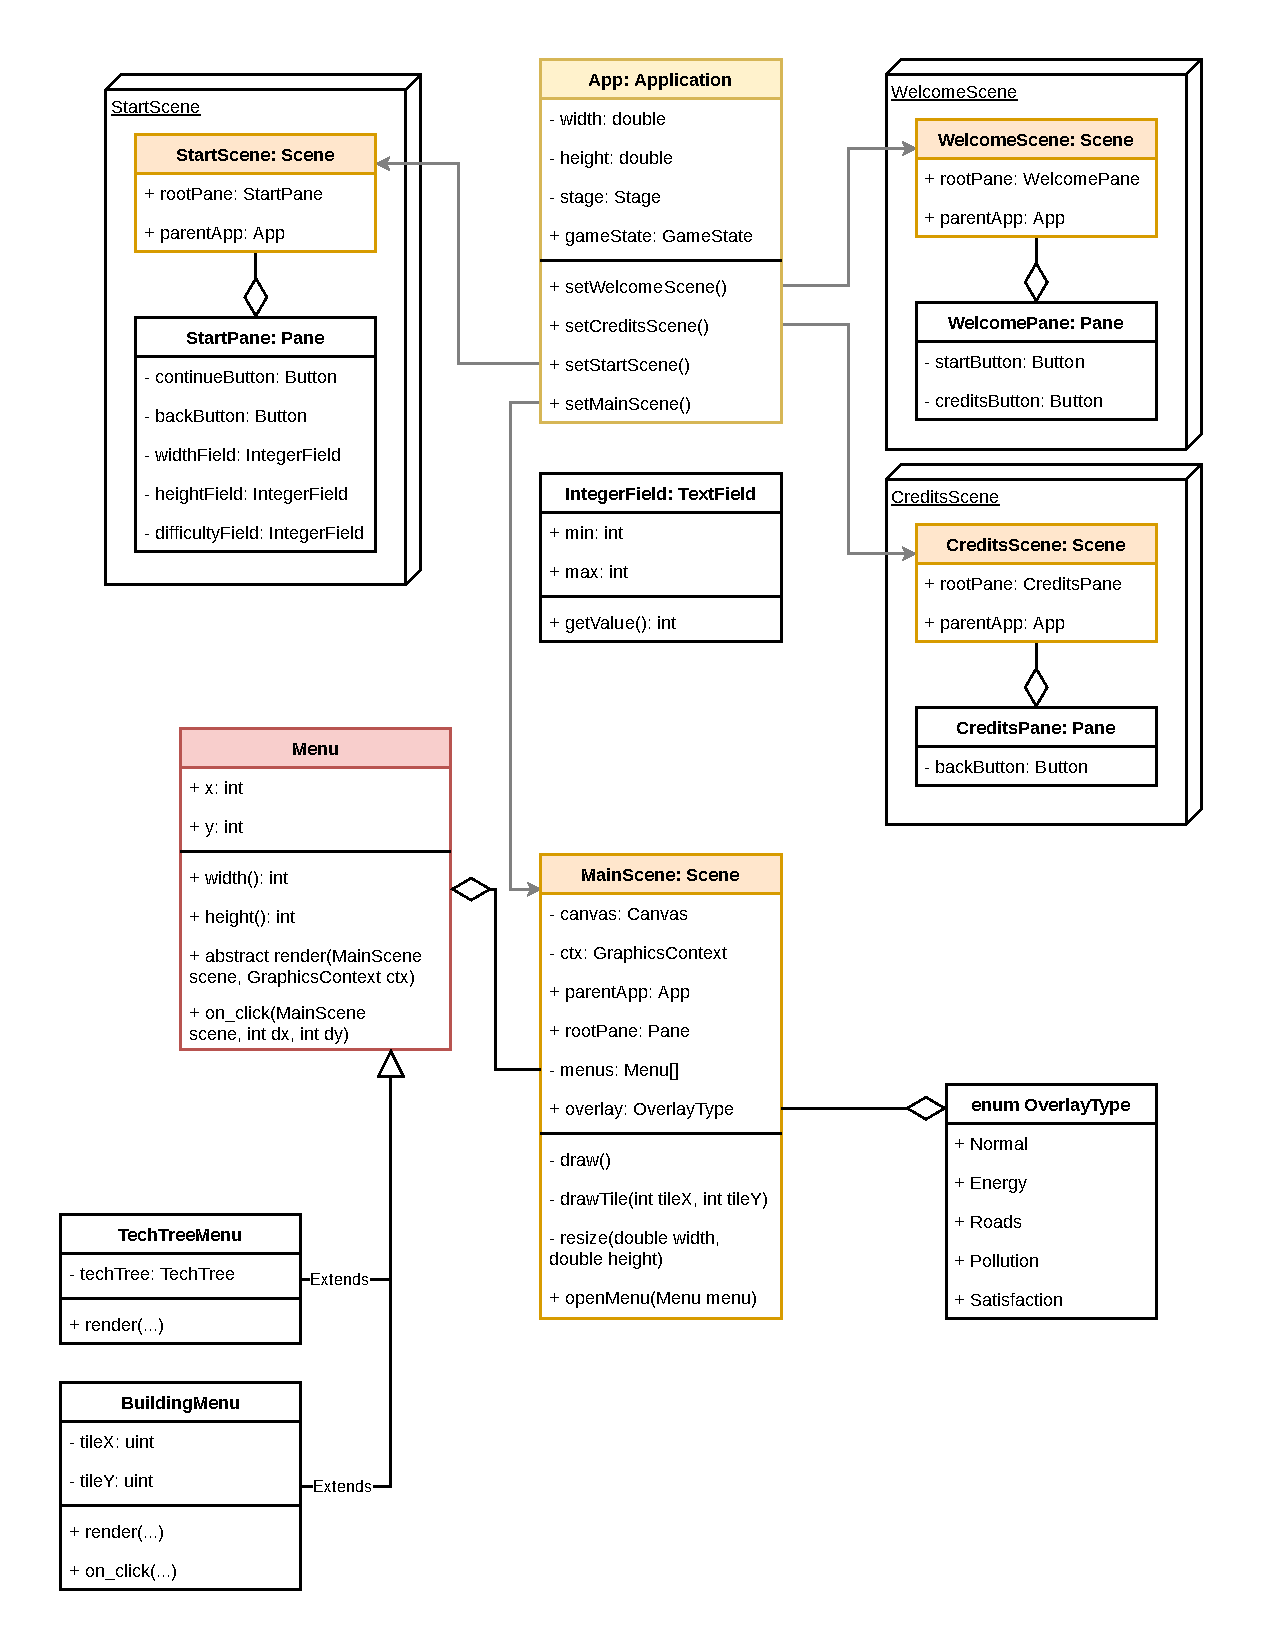
\includegraphics[width=\textwidth]{uml-classes-Page-6}
\caption{La classe \texttt{App} et les différentes classes pour l'affichage du jeu.\label{fig:application}}
\end{figure}

\section{Description Textuelle}

En parallèle du diagramme de classe, nous avons élaboré une description textuelle de certains cas d'utilisation:

\begin{itemize}
    \item Placer un bâtiment
    \item Sélectionner un bâtiment sur la carte
    \item Voir les informations spécifiques à un bâtiment
    \item Supprimer un bâtiment
    \item Améliorer un bâtiment
    \item Débloquer un bâtiment
    \item Créer des habitations aux endroits libres
    \item Connaître les informations détaillées de la ville
\end{itemize}

% Nope, not typing this back out by hand when I only have three hours before the deadline
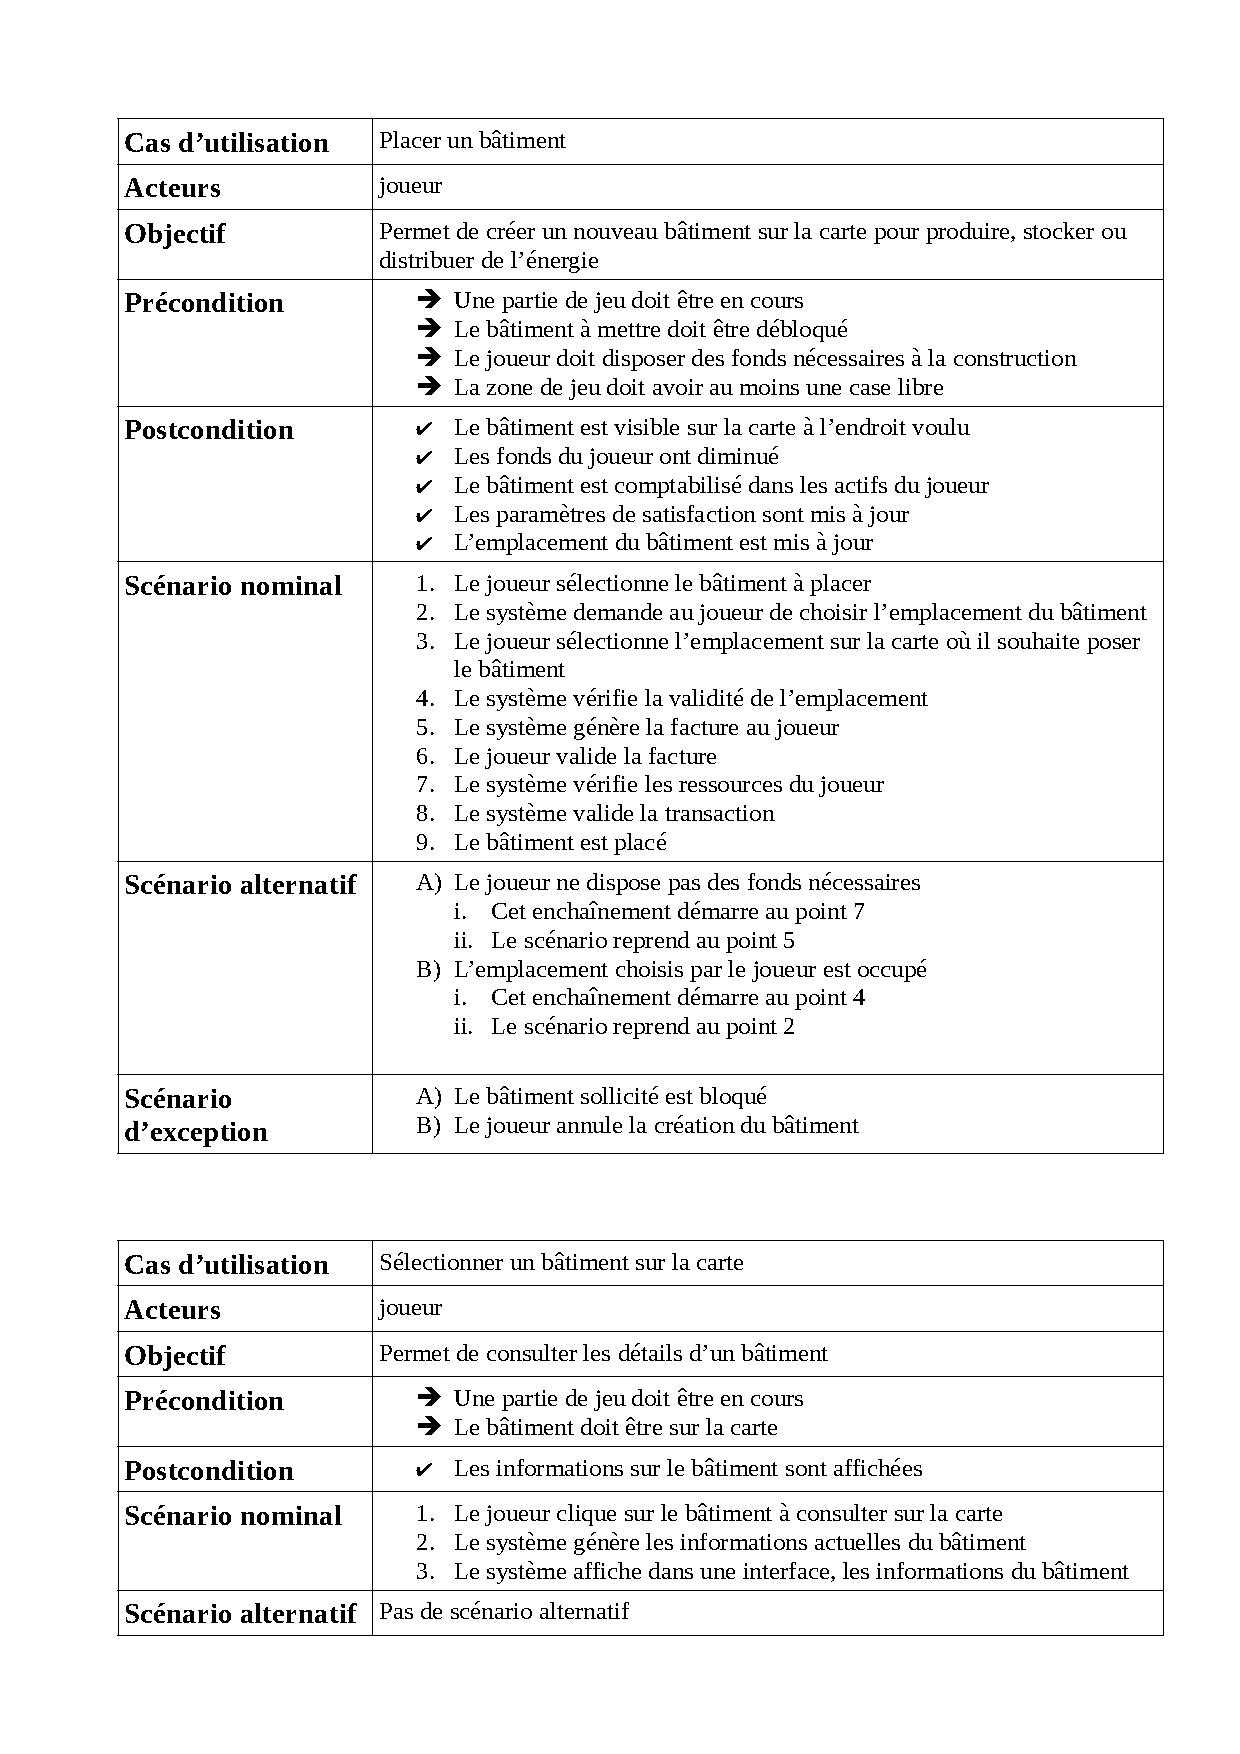
\includepdf[pages=-]{uml-textual-description}

\section{Diagrammes de séquence}

Enfin, nous avons construit quatre diagrammes de séquence, pour détailler l'ordre d'opération des systèmes complexes du jeu:

\begin{itemize}
    \item La fonction \texttt{update()} de \texttt{GameState}, correspondant à une étape de simulation (Figure~\ref{fig:seq-update})
    \item Les actions que le joueur peut faire par rapport aux bâtiments (Figure~\ref{fig:seq-player})
    \item Le fonctionnement de la banque (Figure~\ref{fig:seq-bank})
\end{itemize}

\begin{figure}[H]
    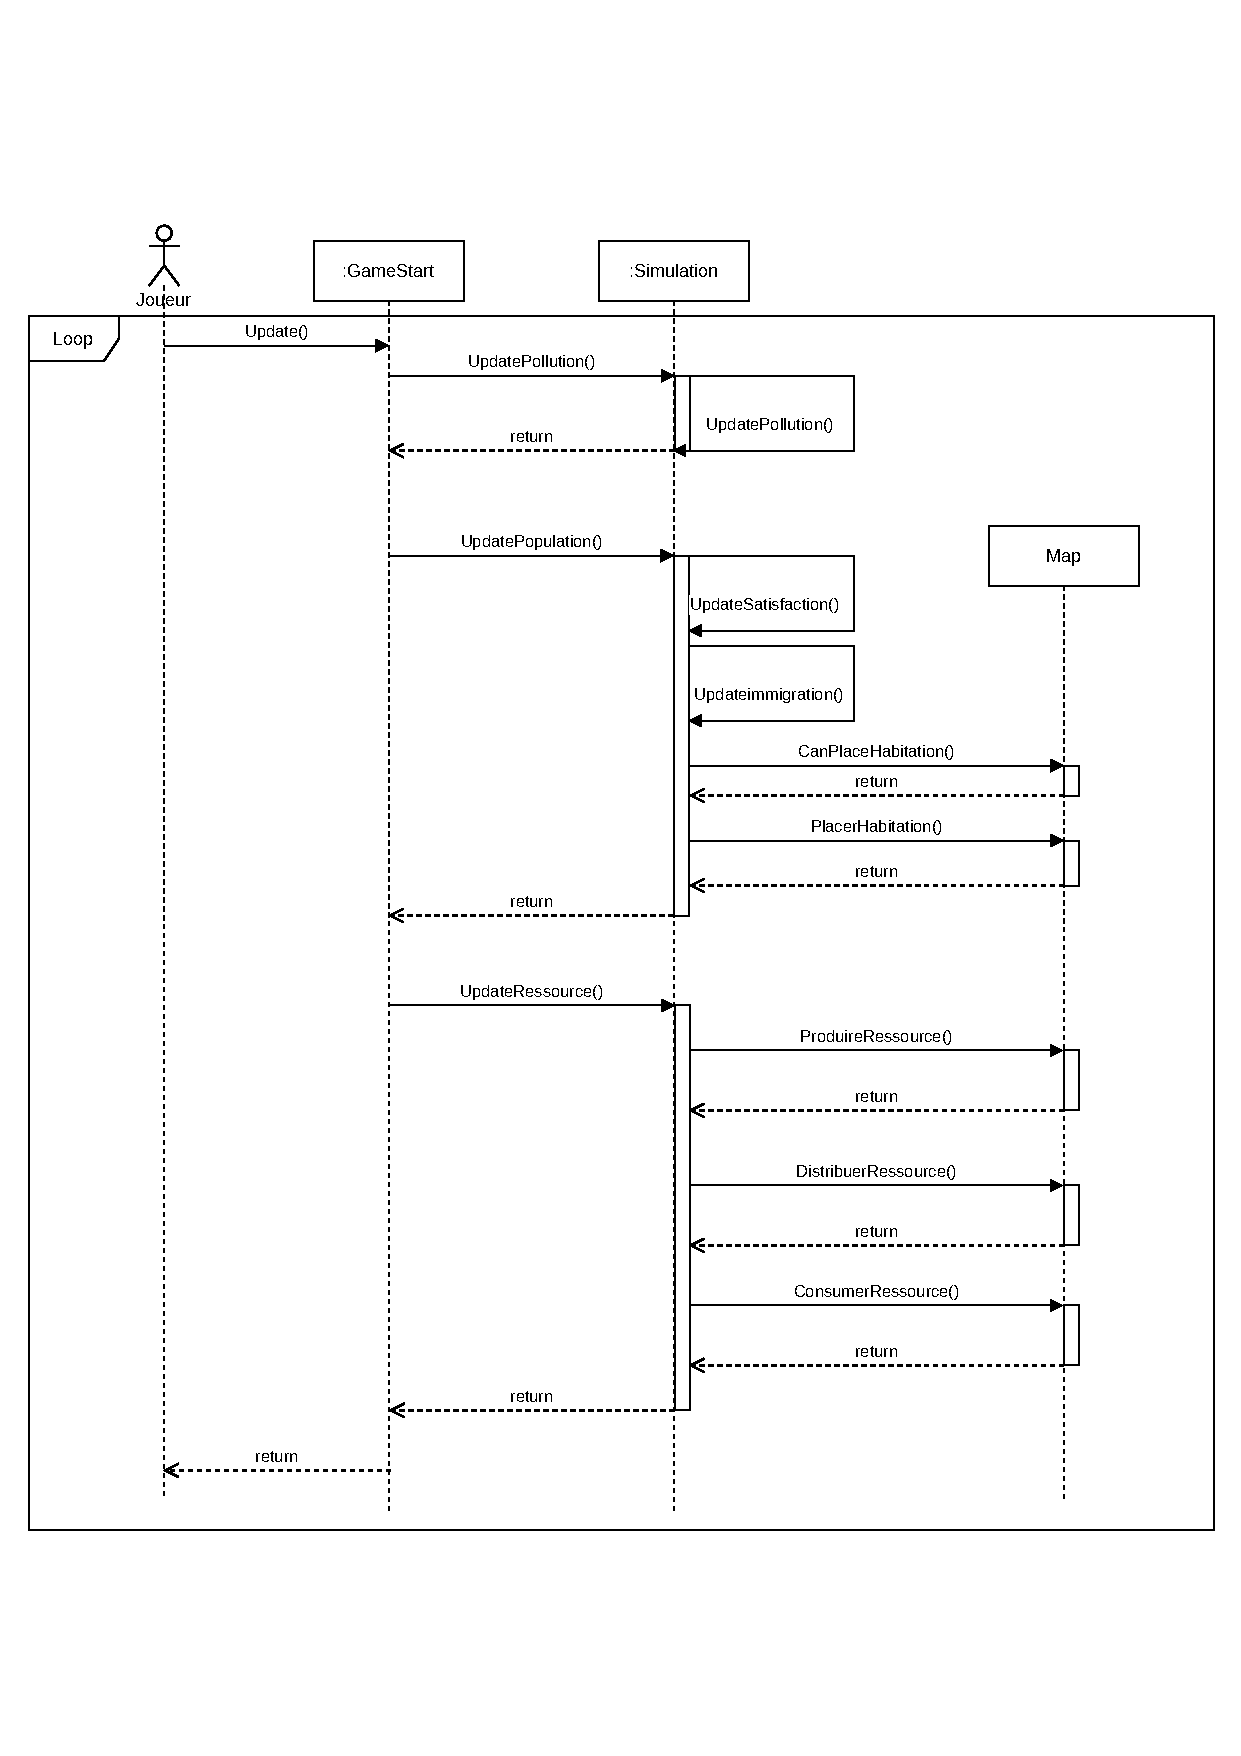
\includegraphics[width=\textwidth]{uml-sequence-1}
    \caption{Diagramme de séquence d'une étape de simulation\label{fig:seq-update}}
\end{figure}

\begin{figure}[H]
    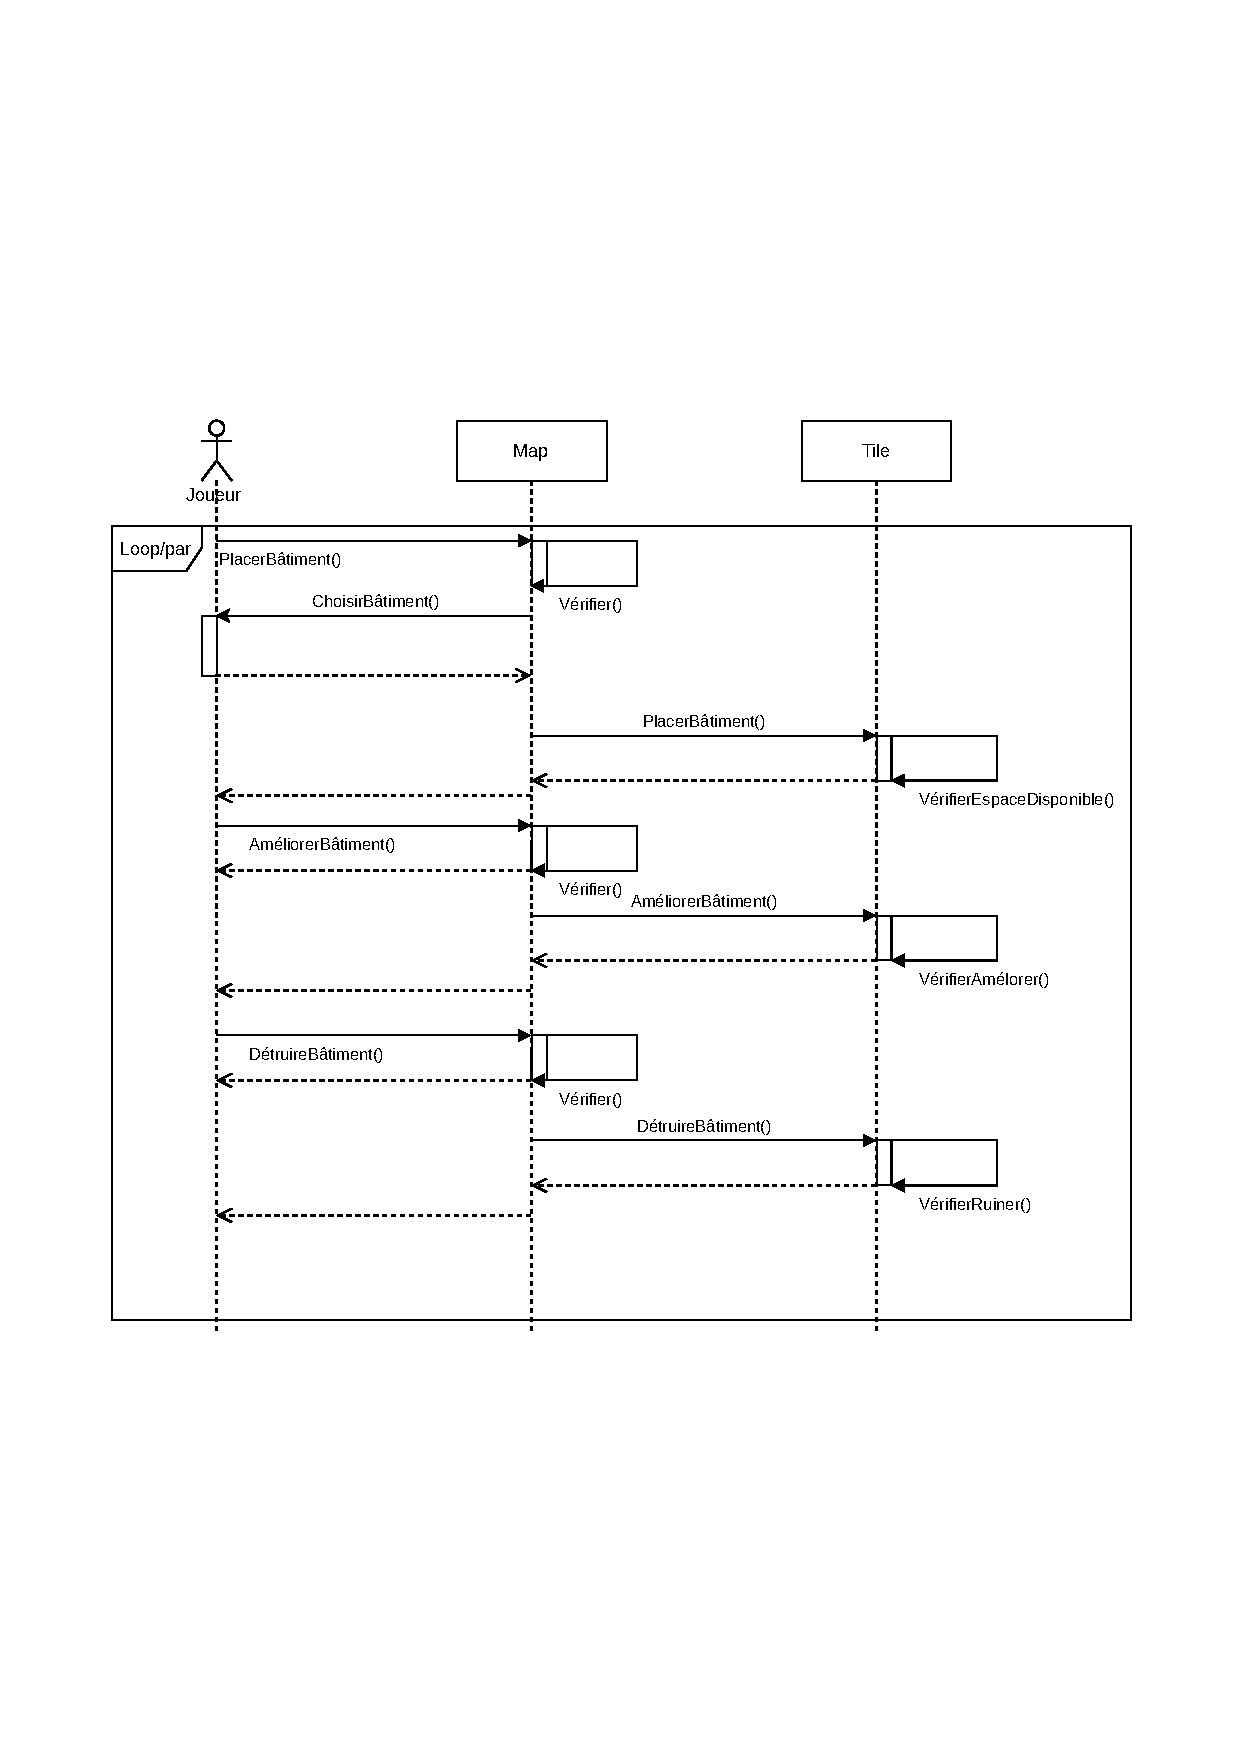
\includegraphics[width=\textwidth]{uml-sequence-2}
    \caption{Diagramme de séquence des actions du joueur sur les bâtiments\label{fig:seq-player}}
\end{figure}

% The 3rd diagram seems to contain no additional data over what's in the first diagram, so I'm skipping it. We hit the page quota already so /shrug

\begin{figure}[H]
    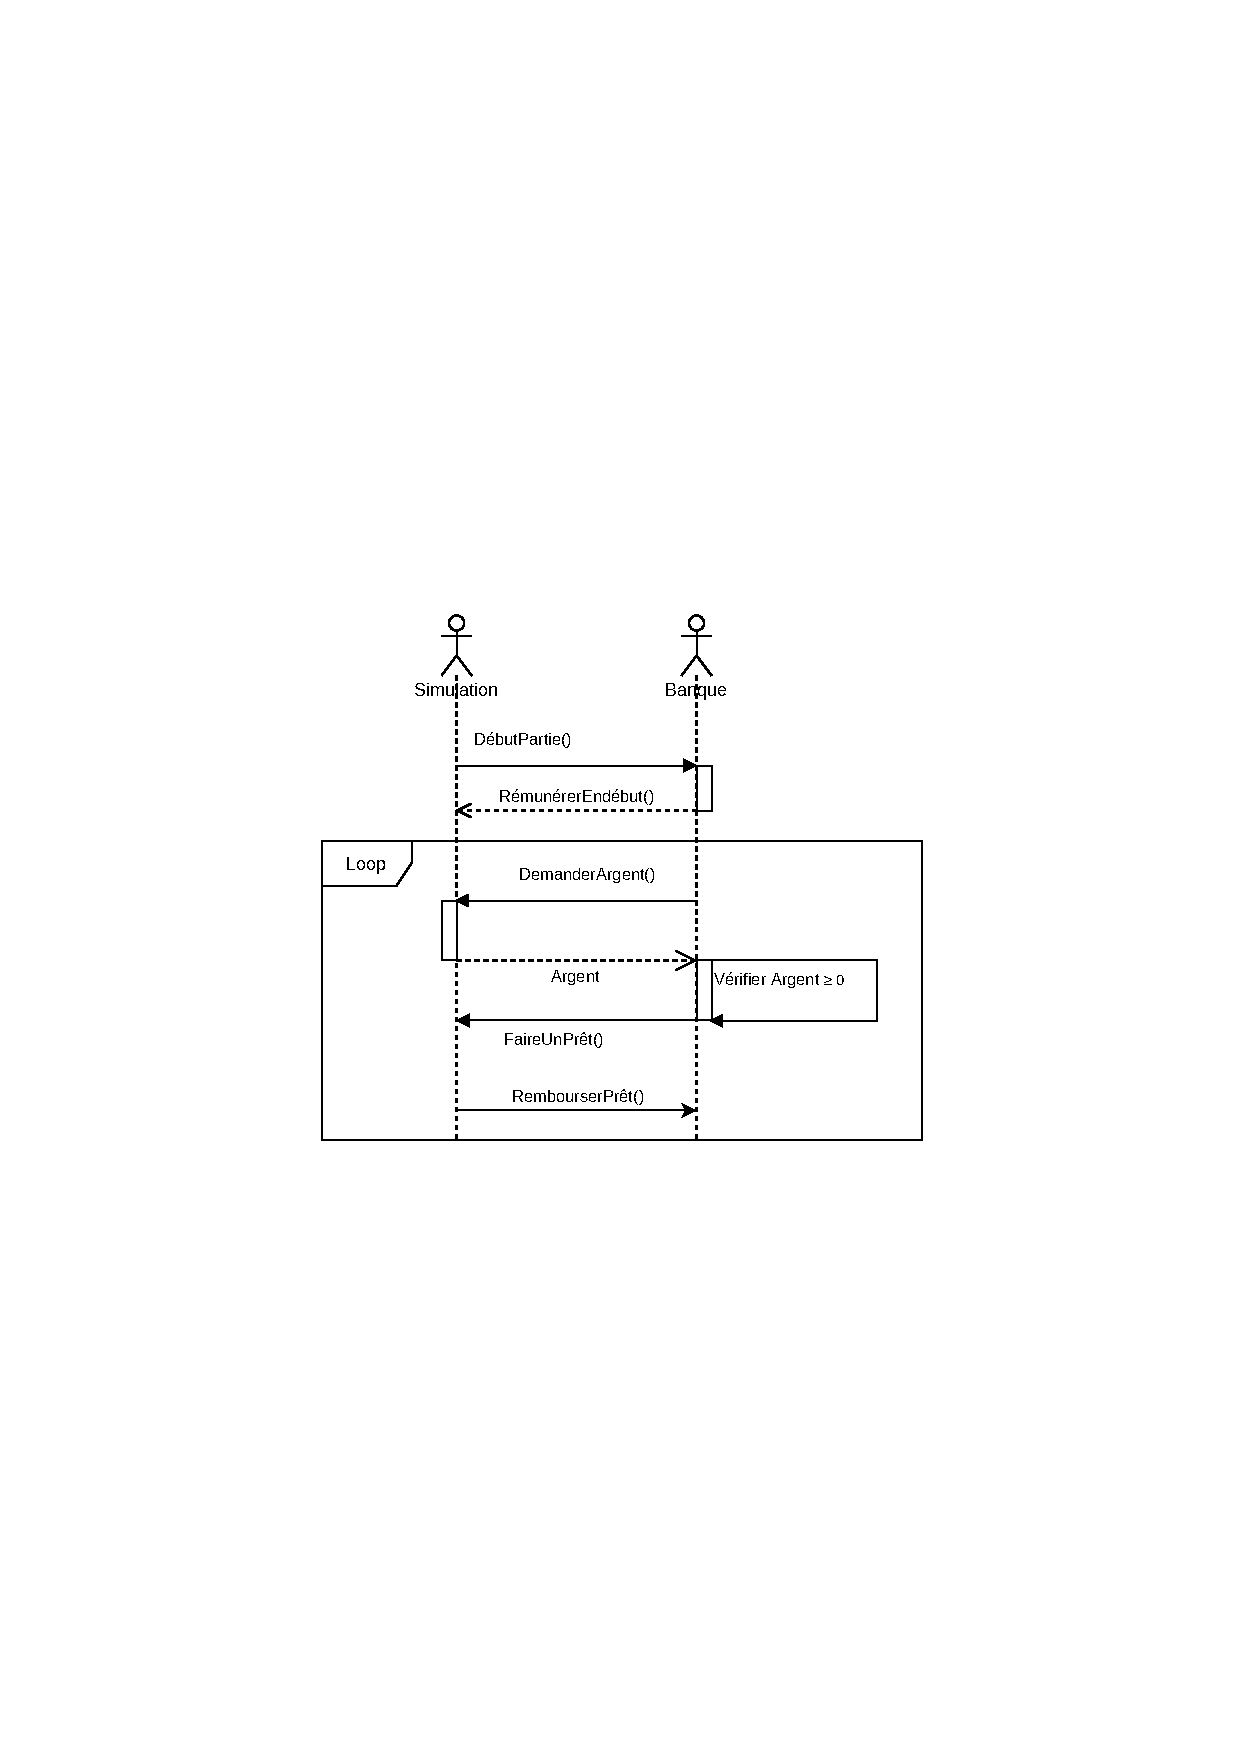
\includegraphics[width=\textwidth]{uml-sequence-4}
    \caption{Diagramme de séquence des actions de la banque\label{fig:seq-bank}}
\end{figure}

\section{Diagramme de communication}

Le diagramme de communication met en avant le sens des communications entre les différents objets constituant le coeur du jeu: le joueur, la simulation, les habitants et la zone de jeu.

\begin{figure}[H]
    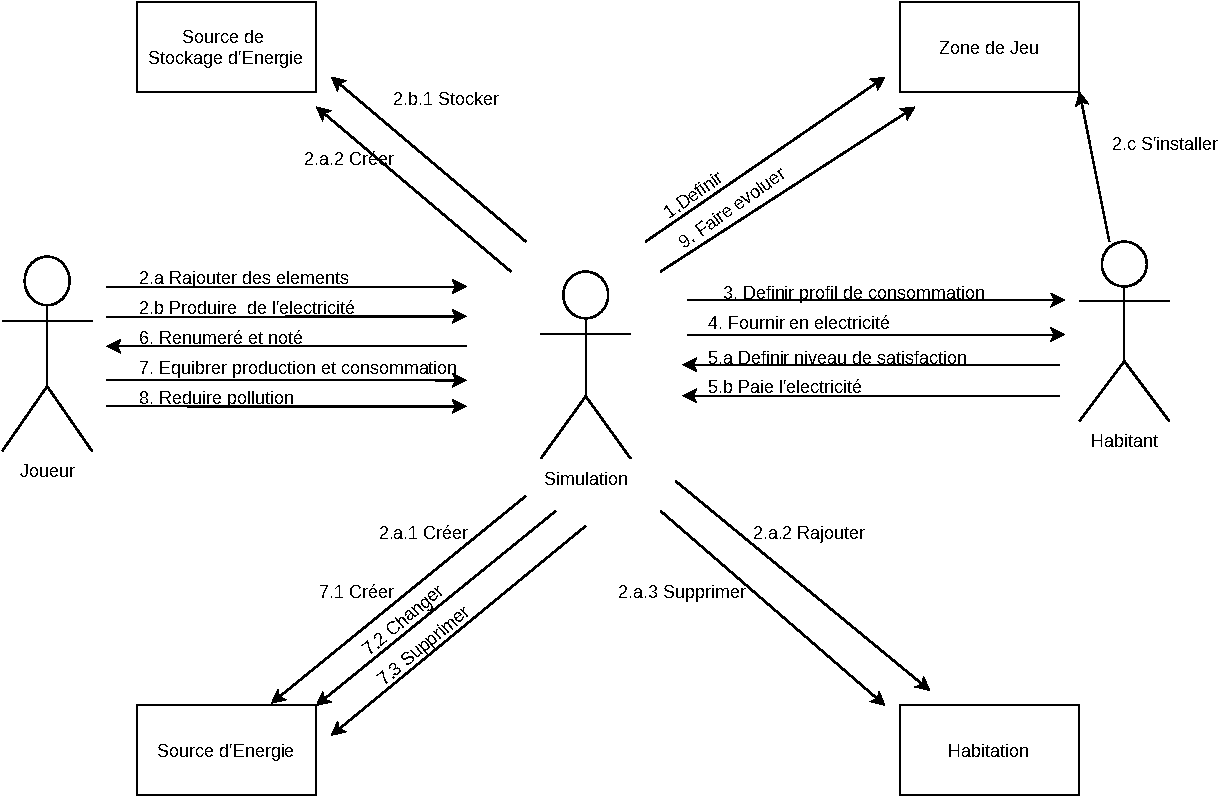
\includegraphics[width=\textwidth]{uml-communication}
    \caption{Diagramme de communication\label{fig:communication}}
\end{figure}

\end{document}
